%!TEX root = ../PTC-LibUG.tex

\chapter{Overview of \PTC}
\label{cha:overview}

%% FiXme
\fxnote{Review underscore (\_\,) characters in index entries.}
\fxnote{Review labels.}
\fxnote{Review use of {\normalfont\texttt{\char`\\index}}.}
\fxnote{Period at end of side refs?}
\fxnote{Justification of margin-float captions.}

\index{PTC!overview}
\index{overview!PTC}
\index{integrator!overview}
\index{geometric transformation!overview}
\index{transformation|see{geometric transformation}}
%
This overview describes the \PTC\ approach to simulating and analyzing
particle accelerators.

At the heart of \PTC's accelerator simulation code is an integrator
capable of tracking particles through various kinds of beamline
elements.  A particle going through a beamline element sees only the
\emph{local} magnetic field, and \PTC\ uses a \emph{local} reference
frame for describing that magnetic field---the frame most appropriate
for the geometry of that type of element.  To track through a series
of beamline elements, \PTC\ locates the elements with respect to each
other using geometric transformations that connect the reference frame
of one element to the reference frame of neighboring elements. Those
two pieces---the integrator and the geometric transformations---give
\PTC\ the capability to model an accelerator with arbitrarily placed
beamline elements.

In tracking orbits through particle accelerators, we want the capability
of modeling not only simple linear and ring accelerators, but also complex
topologies, for example, the Continuous Electron Beam Accelerator Facility
(CEBAF) at the Jefferson National Laboratory (JLab).  To model a complex
topology correctly%
\sidenote{Here \emph{correctly} means ``in a manner that respects the
physical reality''.},
\PTC\ uses a data structure that captures the location of the physical
elements as well as the topology of the beam trajectory.  It is that
data structure that makes it possible for us to modify a \emph{single}
\PTC\ beamline element in our simulation code---even when more than one
distinct beam trajectory traverses that element. See the discussion of
\TSref*{accel.topo}.

\PTC\ itself handles the integrator, the geometric transformations, and
the associated data structures, which provide the capability to track
particle orbits through complex topologies.  Inside of \PTC\ is a set
of modules referred to collectively as the Full Polymorphic Package
(\FPP).%
\cite{Forest:2006:FPP.PTC,Forest:2006:FPPDoc}
These routines extend the capabilities of \PTC, making it possible
not only to track particles, but also to propagate Taylor maps. \PTC\ uses
\FPP\ to compute the maps one may analyze for accelerator properties
of interest to us: lattice functions and the like.
\TSref{analyze.accel.prop} discusses this topic.

Finally, when we track particles in accelerators, we must sometimes
account for particle interactions.
\TSref{ptcl.intxns} discusses this topic.

For in-depth discussions of the topics introduced in this overview,
see the \Bibref, \pref{bib}.


\subsection{\PTC\ and Reference Trajectories}

\index{reference trajectory!not used by PTC}
\index{trajectory!reference}
\index{reference orbit|see{reference trajectory}}
%
A \emph{reference trajectory} or reference \emph{orbit} describes the
ideal path of a particle through an ideal accelerator.  Accelerator
modeling codes that use a reference trajectory simulate particle orbits
as deviations from that ideal. However, a particle traveling through a
real accelerator ``sees'' only \emph{local} magnetic and electric fields,
and \PTC\ respects this physical reality. When pushing a particle through,
say, a quadrupole, \PTC\ makes no distinction between that magnet sitting
on a lab bench and that magnet in a beamline: it simply integrates the
particle motion in a frame local to that quadrupole. As we shall see,
an essential component---perhaps \emph{the} essential component---of
\PTC\ is the collection of geometry routines that handle transformations
between different frames of reference. This approach has the added benefit
that even large displacements---\eg, a quadrupole shifted to act as a
combined-function bend---can be handled in the same consistent and
physically correct manner.


\section{Tracking Particles through an Accelerator}
\label{sec:track.ptcl.accel}

\index{particle!tracking}
%
This section discusses four important concepts that enable
\PTC\ to perform accurate simulations of particles through
an arbitrarily complex accelerator:
\begin{itemize}
  \item blocks,
  \item geometric transformations,
  \item particle tracking,
  \item data structures for modeling accelerator topologies.
\end{itemize}


\subsection{Blocks}
\label{sec:blocks}

\index{integrator!described}
\index{PTC!integrator}
\index{symplectic integrator|see{integrator}}
\index{s-based tracking!described}
\index{magnet-based tracking|see{s-based tracking}}
\index{tracking|see{\emph{also} s-based tracking \emph{or} time-based tracking}}
%
\PTC\ uses the longitudinal co\"ordinate, generically denoted $s$,
as the independent variable for integrating particle trajectories.%
\footnote{\PTC\ also has the capability to perform first-order
time-based tracking. See \TSref*{ptcl.intxns}.}
The particulars of \PTC's $s$-based, or \emph{element}-based, tracking
serve to maintain the physical and mathematical integrity of each
element in a beamline and, moreover, make it possible for \PTC\ to
provide information about particles inside an element, again without
violating the element's physical and mathematical integrity.
To explain how \PTC\ does this, we use an analogy with \LEGOr\ blocks.

\index{LEGO block!analogy}
\index{frame of reference!magnet}
%
Each different type of beamline element in an accelerator is analogous
to a different type of \LEGO\ block in the sense that \LEGO\ blocks are
self-contained objects. A magnet, for example, is a self-contained object
that produces a local field that affects local particle trajectories.
Local geometric considerations (\eg, the shape and symmetry of the
magnetic field) determine the co\"ordinate system and frame of reference
for a local Hamiltonian that describes the magnet.  (We choose the
co\"ordinate system and frame of reference so as to push particles
through the element as simply as possible.)
If individual magnets have conflicting geometries, we patch them together.
In other words, we use local co\"ordinate transformations to connect
particle trajectories between the differing geometries. The rest
of the accelerator does not---and should not---affect our choice of
reference frame for any given beamline element.

\index{local coordinate system!defined}
\index{coordinate system|see{global coordinate system \emph{or} local coordinate system}}
\index{reference frame!described}
\index{entrance reference frame!described}
\index{entrance frame|see{entrance reference frame}}
\index{element frame|see{element reference frame}}
\index{element reference frame!described}
\index{exit reference frame!described}
\index{exit frame|see{exit reference frame}}
%
\newthought{A local co\"ordinate system} attached to each beamline
element permits us to propagate physical quantities across the
elements. That internal structure is the province of the integrator.
In addition, each element includes three \emph{reference frames}:
  a reference frame at the entrance,
  a reference frame at the midpoint (the \emph{element} reference frame),
  and a reference frame at the exit. See \fref{LEGO.element}.
These extra frames, used by \PTC\ when it hands a particle from one
element to the next, allow \PTC\ to handle arbitrary changes in the
placement of beamline elements. On entering an element, a particle has
a certain phase-space location with respect to the entrance frame.
\PTC\ tracks the particle as it traverses the element, computing the
particle's phase-space co\"ordinates with respect to the element's exit
frame. Knowing the relation between the exit frame of the current element
and the entrance frame of the subsequent element, \PTC\ uses the
transformations of
the dynamical Euclidean group\cite{Forest:1997:DynEuclid}
to hand the particle to the next element.
\begin{figure}[ht]
  \centering
  \includegraphics[width=0.5\textwidth]%
    {illustrations/LEGO-element-ref-frame}
  \caption{\LEGO-block element, with reference frames for the
           entrance, element body, and exit.}
  \label{fig:LEGO.element}
\end{figure}

\index{drift!defined}
\index{element!drift}
%
The beamline element represented in \fref{LEGO.element} is a
\emph{drift}: a block with parallel entrance and exit faces to
which local Cartesian reference frames are attached. The entrance
and exit reference frames have the same unit vectors. The line that
links the two frames has a length $L$, and it is perpendicular to
both those frames. Note that for the purposes of this discussion,
any beamline element (quadrupole, sextupole, solenoid, \etc) that
does not bend the design orbit is a drift.

\index{bend!defined}
\index{element!bend}
%
A \LEGO-block element might also be a \emph{bend}: a block with two
faces that have parallel $y$-axes (vertical), and $x$-axes (horizontal)%
\marginnote[-12pt]{Note that calling the $x$ and $y$ axes ``horizontal''
and ``vertical'' reflects the bias of accelerator physicists towards
flat rings with vertical dipole fields. What we locally (\ie, within
the element) call the $x$ axis need not be horizontal. See, for example,
the discussion of the vertical bend indicated in \fref{connect.blocks}.}
that meet at an angle $\theta$. The two $x$-axes and the line joining
the two origins form a plane perpendicular to the two faces. An arc
of circle of length $L$ passes perpendicularly through the origin of
both faces. The purpose of this element is to bend an incoming
particle trajectory by approximately angle $\theta$. The internal
details of the element---whether it is a sector bend, a bend with
an irregular field, \etc---is, for this discussion, immaterial.

\begin{marginfigure}
  %\includegraphics[width=\textwidth]{illustrations/LEGO}
  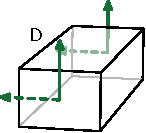
\includegraphics{Blocks/blocks-01}\\ \noindent
  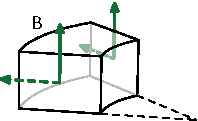
\includegraphics{Blocks/blocks-02}
  \caption{Two \LEGO\ blocks: drift (\ptcelm{D}) and bend (\ptcelm{B}).}
  \label{fig:LEGO.BandD}
\end{marginfigure}

\fref[c]{LEGO.BandD} illustrates these two fundamental types of
\LEGO\ blocks with the entrance and exit reference frames for their
\emph{local} co\"ordinate systems. The solid arrows show the direction
of the local $y$-axes and the dashed arrows show the direction of the
local $x$-axes.
In summary, the bend is characterized by a bending radius $\rho$,
a length $L$, and two faces, each with a reference frame.  The
drift is characterized by a length $L$ and also two faces, each
with a reference frame. The bend is the fundamental block used in
the composition of complex blocks; the drift, of course, is just a
special case of the bend.

\newthought{We are interested} in the deterministic motion through
each \LEGO\ block, represented by the transformation
\begin{equation}\label{eq:zin.zout}
  z_\text{in} \mapsto z_\text{out} = f(z_\text{in}),
\end{equation}
where $f$ denotes a vector of generally nonlinear functions
connecting the local phase-space co\"ordinate $z_\text{in}$
defined in the entrance frame, to the local phase-space
co\"ordinate $z_\text{out}$ in the exit frame. The construction
of such a transformation depends on internal considerations
that are not needed for an understanding of the \LEGO-block
approach. The \LEGO\ block for a single element might, in fact,
comprise a sequence of simpler blocks. This structure, dictated
by the internal geometry of the element, may be hidden.

\begin{marginfigure}[\baselineskip]\forceversofloat
  \centering
  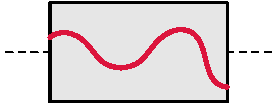
\includegraphics[width=\textwidth]{Blocks/blocks-03}\\[1.5ex]
  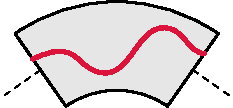
\includegraphics[width=.75\textwidth]{Blocks/blocks-04}
  \caption{Particle trajectories through ``drift'' and ``bend''
           \LEGO\ blocks.}
  \label{fig:LEGO.maps}
\end{marginfigure}
%\begin{figure}[ht]
%  \centering
%  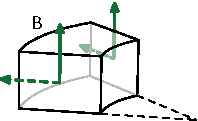
\includegraphics[width=0.6\textwidth]{Blocks/blocks-02}
%  \caption{Particle trajectories through ``drift'' and ``bend''
%           \LEGO\ blocks.}
%  \label{fig:LEGO.maps}
%\end{figure}
In \fref{LEGO.maps} we show a pair of particle trajectories,
in drift and bend \LEGO\ blocks, passing from the entrance face
through to the exit face. As suggested by the trajectories
illustrated, the internal structure may be very complicated
(think of a wiggler); but seen from the outside, our
\LEGO\ blocks are, quite simply, \emph{blocks} with two faces
that define local co\"ordinates with respect to which one may
define $z_\text{in}$ and $z_\text{out}$---\emph{nothing more}.

\index{particle dynamics!local}
\index{element!defined}
\index{beamline element|see{element}}
%
A beamline element is defined by a block with three reference frames,
together with a model, or integrator, which describes how to propagate
a particle from the face with the entrance reference frame to the face
with the exit reference frame:
\begin{equation*}
  \text{element} = \text{block} + \text{model}.
\end{equation*}
The model transforms the phase-space variables from entrance to
exit of the block according to \eqref{zin.zout}. In other words,
it represents the \emph{physics} of the device. Note that the model
also incorporates any approximations we make.

\index{fringe field!magnet}
%
As an example, a block with a bend geometry might actually be a
simple drift, keeping the transverse momenta invariant and
changing only the positions. Or it might be a composition of
blocks describing the body of a magnet and its fringe field
regions. An element might also have non-Hamiltonian effects
such as radiation.%
\footnote{\Aref[c]{states} discusses \PTC's internal state variables,
which describe the characteristic dynamics you can choose for your
accelerator model.}
The list of possible models is endless. In general, a model is
defined by
\begin{itemize}
  \item one or more blocks internal to the model;
  \item a model for each internal block;
  \item the equation of motion in each internal block together with
its integration method and associated number of integration steps.
\end{itemize}

\newthought{In summary}, we define a beamline element locally:
the definition, whether the element is on a work bench or in an
accelerator, is determined solely by the characteristics of that
element. And once we have defined a model for our element, we stick
with it: the \LEGO\ block is inviolate. Like a physical magnet, it
exhibits identical properties under identical conditions.
A significant virtue of our computer-based element, however,
is that it is free to report about what is happening inside.


\subsection{Geometric Transformations}

\index{geometric transformation!defined}
\index{reference frames!connecting}
%
Now that we have defined our two basic types of beamline elements
(drift and bend), the next step is to fit them together. We need
geometric transformations that connect the exit reference frame of
one beamline element to the entrance reference frame of a subsequent
element.

\index{geometric transformation!defined}
\index{LEGO block!analogy}
\index{global frame!described}
\index{global coordinate system!global frame}
\index{layout!global frame}
%
Continuing the \LEGO-block analogy, we put the individual
\LEGO\ blocks on a base, which represents the accelerator model's
\emph{global frame}. Once we know the location of each
\LEGO\ block with respect to the global frame, we know their
locations with respect to to one another.
\fref[c]{LEGO.blocks.base} shows two such \LEGO\ blocks and
their reference frames on a base, which represents the layout of
beamline elements in the global frame of an accelerator. With the
\LEGO\ blocks now on the global frame, we require transformations
that translate the phase-space co\"ordinates in the exit reference
frame of one \LEGO\ block to the phase-space co\"ordinates in the
entrance reference frame of the next \LEGO\ block.
\begin{figure}[ht]\forcerectofloat
  \centering
  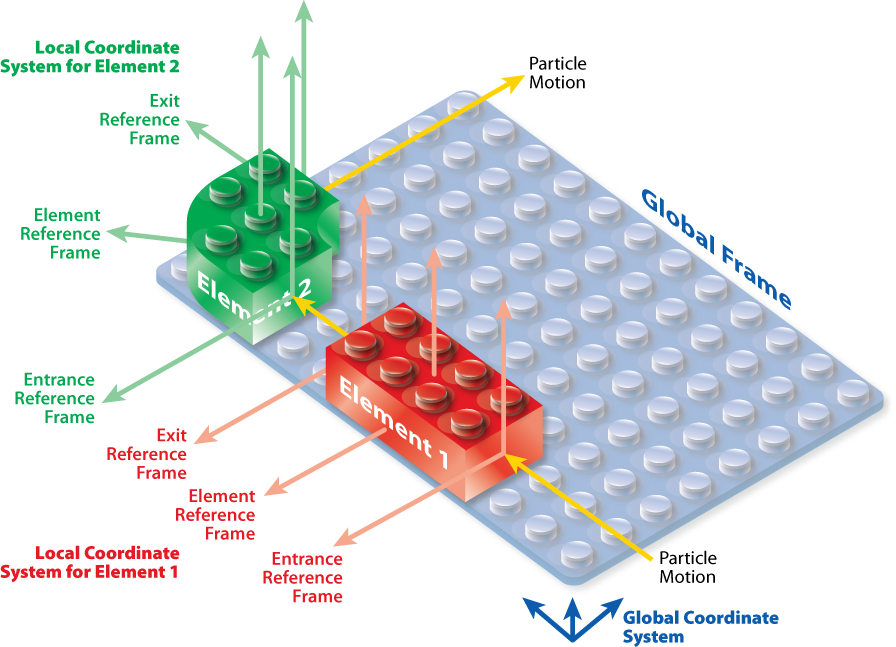
\includegraphics[width=.9\textwidth]{illustrations/LEGO-concept-2}
  \caption{Two \LEGO\ blocks (elements) on a base (global frame).}
  \label{fig:LEGO.blocks.base}
\end{figure}

To construct, for example, a recirculating accelerator out of
\LEGO\ blocks, we connect bends and drifts one after another to
model the desired machine. On reaching the last \LEGO\ block,
we require that the last block's exit face coincide with the
first entrance face. This means that
\begin{itemize}
  \item the blocks' faces must be parallel;
  \item and the frames on the two faces must line up.
\end{itemize}

\begin{marginfigure}[-2.5\baselineskip]
  %\includegraphics[width=\textwidth]{illustrations/connecting-blocks}
  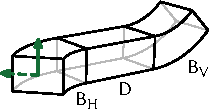
\includegraphics{Blocks/blocks-05}\\
  \noindent\hspace*{.8em}
  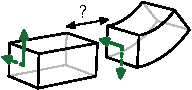
\includegraphics{Blocks/blocks-06}
  \caption{Connecting two horizontal \LEGO\ blocks and a vertical
           \LEGO\ block.}
  \label{fig:connect.blocks}
\end{marginfigure}

\index{patching!defined}
%
Connecting a horizontal bend with a horizontal drift, as for
elements $\text{\ptcelm{B}}_\text{\ptcelm{H}}$ and \ptcelm{D}
in \fref{connect.blocks}, is easy because the $x$- and $y$-axes
of the two elements match. Connecting a horizontal drift with
a vertical bend, as for elements \ptcelm{D} and
$\text{\ptcelm{B}}_\text{\ptcelm{V}}$ in \fref{connect.blocks},
is not as straight-forward: their local $x$- and $y$-axes do not
match. We need, in essence, a new type of
\LEGO\ block---one with an $x$-$y$ rotation of angle $\phi$. (In
\fref{connect.blocks}, of course, $\phi=\ang{90}$.) To build an
arbitrary accelerator, we shall require a full complement of such
additional \LEGO\ blocks.%
\cite[15pt]{Forest:1997:DynEuclid}
This is the subject of \emph{patching}, which uses geometric
transformations to connect the exit frame of one beamline element
to the entrance frame of a subsequent element. Most significantly,
patching enables us to position beamline elements wherever we want
them. We discuss this in more detail later in \TPref*{sec:chart.patch}.

\subsection{Particle Tracking}
\label{sec:ptcl.track}

Now that we have the basic building blocks and the geometric
transformations to fit them together, we can begin to think about
how to track particles. Here we present some essential information
about particle tracking in \PTC.

In keeping with its \LEGO-block philosophy, \PTC\ tracks particles
with respect to \emph{local} frames of reference. The local phase-space
co\"ordinates together with \PTC's knowledge of the local frames
allow the interested user to reconstruct full 3D particle
trajectories with respect to the global frame. In fact, doing exactly
that is useful for checking that one has the constructed the correct
lattice topology in \PTC.

\newthought{Units:} PTC measures all lengths in meters, and all
angles in radians. (It provides the constant \ptc{twopi} to simplify
the conversion from degrees.%
\sidenote{Many other constants are defined in the module
\ptcmod{precision\_constants}.})
Particle momenta are scaled by a value $p_o$. This scale momentum
is usually set when defining the lattice (see, for example,
the discussion of \ptc{set\_mad} on
\pref{set.mad}). A subtle point involves the fact that the scale
set for one element may differ from that in the preceding element,
\eg\ in the case of acceleration.
In such cases, the patching mentioned above must include not only
geometric transformations, but also energy transformations.

\newthought{Tracking State:} \PTC\ defines a variable
type called \ptctyp{internal\_state}.
Objects of this type may be used to modify certain assumptions
\PTC\ makes when it performs tracking. One may, for example,
ask \PTC\ to track only the 4D transverse phase-space variables;
or one may turn on or off radiation. A variable of type
\ptctyp{internal\_state}
is essentially a list of flags that one may pass to \PTC\ tracking
routines to modify the algorithms used. For more information, see
\TAref*{states}.

\index{phase space!variables}
\index{variable!phase space}
%
\newthought{Phase-Space Co\"ordinates:} With the default tracking
state, \PTC\ uses the six phase-space variables%
\sidenote{\PTC\ can turn all six of the variables into Taylor series,
or it can omit two of them.  Setting an \ptctyp{internal\_state} flag
to ``only four dimensions'' implements the latter behavior.}
\fxnote{Add reference to use of \textsc{only\_4d}.}
\begin{subequations}\label{eq:vars.dev}
\begin{equation}\label{eq:vars.dl}
  (x, p_x,\, y, p_y,\, \delta, \ell).
\end{equation}
Here $x$ and $y$ denote the \emph{local} transverse co\"ordinates,
and $p_x$ and $p_y$ denote the corresponding canonical momenta
(divided by a scale momentum $p_o$). The fifth variable, $\delta$,
denotes the relative momentum deviation
\begin{equation*}
 \delta = \frac{p - p_o}{p_o};
\end{equation*}
and the sixth variable, $\ell$, denotes the path-length deviation.%
\sidenote{These last two variables are kept in this order for a technical
reason. This ordering allows us to retain the natural meanings:
positive $\delta$ implies higher energy, and positive $\ell$ implies
longer path length. Because of the Hamiltonian structure, reversing
their order would require us to reverse the sign on one of them.}

One may modify the tracking state so as to change the phase-space
variables. If desired, one may set a flag that causes \PTC\ to compute
flight time rather than path length. In this case, the phase-space
co\"ordinates are
\begin{equation}\label{eq:vars.et}
  (x, p_x,\, y, p_y,\, \varepsilon, ct).
\end{equation}
\end{subequations}
Here the fifth variable, $\varepsilon$, denotes the scaled energy
deviation
\begin{equation*}
  \varepsilon = \frac{E - E_o}{p_o c},
\end{equation*}
where $E_o$ is the energy associated with $p_o$. (In other words, if
$p_o = m c^2 \beta_o \gamma_o$, then $E_o = m c^2 \gamma_o$.) And
the sixth variable, $ct$, is the time-of-flight deviation multiplied by
the speed of light.

One may set a separate flag that causes \PTC\ to compute the total
path length (or flight time) rather than the deviation. In this
case the phase-space variables will be either
\begin{subequations}\label{eq:vars.tot}
\begin{equation}\label{eq:vars.dL}
  (x, p_x,\, y, p_y,\, \delta, L),
\end{equation}
or
\begin{equation}\label{eq:vars.eT}
  (x, p_x,\, y, p_y,\, \varepsilon, cT),
\end{equation}
\end{subequations}
where $L$ and $T$ denote respectively the \emph{total} path length and
\emph{total} flight time.

\begin{marginfigure}[4\baselineskip]\forceversofloat
  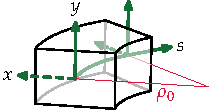
\includegraphics{Blocks/blocks-22}
  \caption{Geometry and local co\"ordinates, $(x,y,s)$, for a
           generic block in \PTC.}
  \label{fig:block.coords}
\end{marginfigure}

\newthought{Hamiltonians:} In accord with its \LEGO-block philosophy,
\PTC\ tracks a particle across an element using a Hamiltonian that is
\emph{local} to that element. The Hamiltonian used by \PTC\ in the body
of an element (no fringe field) then has the simple form
\begin{subequations}\label{eq:Hams}
\begin{equation}\label{eq:Ham.dL}
  - (1 + \kappa_o x) \sqrt{\vphantom{()}\smash{
                           (1 + \delta)^2 - p_x^2 - p_y^2}}
  + (1 + \kappa_o x) \frac{q}{p_o} A_s(x,y)
\end{equation}
if one uses the variables \eqref{vars.dL}, or
\begin{equation}\label{eq:Ham.eT}
  - (1 + \kappa_o x) \sqrt{\vphantom{\frac{1}{1}}\smash{
                           1 + \frac{2}{\beta_o}\,\varepsilon
                             + \varepsilon^2 - p_x^2 - p_y^2}}
  + (1 + \kappa_o x) \frac{q}{p_o} A_s(x,y)
\end{equation}
\end{subequations}
if one uses the variables \eqref{vars.eT}.
Here $\kappa_o = 1 / \rho_o$ denotes
the curvature defined by the \emph{geometry} of the element, and
$A_s$ denotes the longitudinal component of the vector potential.
\fref[c]{block.coords} indicates the variables, including the longitudinal
co\"ordinate $s$. That figure indicates a horizontal bend;
for vertical bends, we do as indicated in the lower part of
\fref{connect.blocks}.
For straight elements, of course, $\kappa_o=0$. If one uses the
variables \eqref{vars.dev}, then there is, effectively, an
additional term that subtracts the default path length or flight
time across that element.\cite{Barber:1994:SpinI}

One may, if desired, have \PTC\ track using an approximation of one of
the Hamiltonians \eqref{Hams} (\ie, using truncated expansions for the
square-root and the vector potential). One might,
for example, do this to speed the computation, but of course the
validity of the expansion for your particular problem should be
verified with careful testing.

\fxnote{Consider using natbib.}
\fxnote{Add reference to \ptc{exact=.false.}}
\fxnote{Add references to use of \textsc{drift\_kick\_drift} and
\textsc{mad\_kind}.}

When integrating across an element described by one of the
Hamiltonians \eqref{Hams}, one typically splits the Hamiltonian
into two integrable pieces.%
\cite{McLachlan:2002:SplitMeth}
If those pieces are, for example, the two terms of \eqref{Ham.dL},
then this is referred to as a \emph{drift-kick} split. Since the
motion of a particle in a uniform dipole is integrable, an
alternative split involves writing $A_s(x,y)$ as a sum of two
pieces: the part that produces a uniform dipole field, and everything
else. Then the dipole field part is added to the drift term of
the Hamiltonian, and we obtain a \emph{bend-kick} split.%
\cite{Forest:1998:BeamDyn,Forest:2006:GeomIntegPA}
One may ask \PTC\ to use one or the other of these splitting methods.

\newthought{Structures for Particles and Beams:} Because \PTC\ tracks particles
with respect to local frames of reference, a set of values for
(as an example) the six phase-space variables \eqref{vars.dl} will not mean
too much unless one knows the context---in particular, where in
the lattice the particle is located. When you need \PTC\ to keep
track of such information for you, it provides some additional
structures. The type \ptctyp{beam} holds an $N\times6$ array for the phase-space
variables, as well as a pointer that tells you where in the lattice
that beam is located. There is also a type \ptctyp{probe} that holds not only
phase-space data, but also data about a particle's spin state.


\subsection{Data Structures for Modeling Accelerator Topologies}

\index{data structure!modeling accelerators}
\index{accelerator topology!simple}
\index{accelerator topology!complex}
\index{topology|see{accelerator topology}}
\index{accelerator!modeling}
\index{modeling!accelerator topologies}
%
\PTC\ data structures fully account for the three-dimensional
structure of a lattice and potential topological complexities
such as those found in colliders and recirculators. In this section,
we discuss a simple lattice and then two complex lattices.

\begin{marginfigure}[0\baselineskip]\forcerectofloat
  \centering
  %\includegraphics[width=\textwidth]{illustrations/model-simple}
  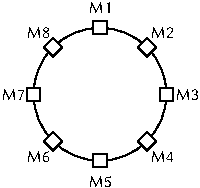
\includegraphics{Layouts/layouts-01}
  \caption{Forward propagation of particles in a circular accelerator.}
  \label{fig:accel.simple}
\end{marginfigure}

\index{forward propagation!example}
\index{propagation|see{backward propagation \emph{or} forward propagation}}
\index{linked list!example for magnets}
%
{A very simple lattice} is shown in \fref[c]{accel.simple},
which illustrates basic forward propagation of particles through a
sequence of magnets%
\marginnote[5pt]{In this discussion, we use the word
``magnet'' whether or not it is actually a magnet, a drift, or any
other beamline element.}
that never varies. Each magnet appears once in the sequence, and
particles go magnet-to-magnet from \ptcelm{M1} through \ptcelm{M8}.
At that point, they re\"enter the magnet \ptcelm{M1}.
A simple linked list of magnets suffices to model this basic topology:
\begin{equation*}
  \text{\ptcelm{ring}} = \text{linked-list}(\text{%
    \ptcelm{M1}, \ptcelm{M2}, \ptcelm{M3}, \ptcelm{M4},
    \ptcelm{M5}, \ptcelm{M6}, \ptcelm{M7}, \ptcelm{M8}}).
\end{equation*}
One might instead use an array of magnets, but that approach
would require us to recreate and reallocate the array whenever
we wish to add or insert a new element. A virtue of the linked
list is that one may easily add or rearrange elements in the
lattice. However, such a simple approach does not suffice when
an accelerator topology reuses the magnets in different sequences,
different directions, or both.

\index{accelerator topology!recirculating}
\index{recirculator!example}
\index{Continuous Electron Beam Accelerator Facility!example based on}
\index{CEBAF|see{Continuous Electron Beam Accelerator Facility}}
\index{Thomas Jefferson National Laboratory!example based on}
\index{JLab|see{Thomas Jefferson National Laboratory}}
%
{To see the difficulties associated with a recirculating beam},
consider \fref[c]{accel.CEBAF}, which shows a machine similar
to the Continuous Electron Beam Accelerator Facility
(\CEBAF) at Thomas Jefferson National Laboratory (\JLab). It
illustrates the concept of particles circulating through a varying
sequence of magnets. The particles start out traveling through an
injector from magnet \ptcelm{M1} through magnet \ptcelm{M4}.
During the first trip circulating around the accelerator, the
particles go through the sequence of magnets \ptcelm{M5},
\ptcelm{M6}, \ptcelm{M7}, \ptcelm{M8}, \ptcelm{M9}, \ptcelm{M10},
\ptcelm{M11}, and \ptcelm{M12}. During their second trip around
the accelerator, the particles go through the sequence of magnets
\ptcelm{M5}, \ptcelm{M6}, \ptcelm{M13}, \ptcelm{M14}, \ptcelm{M9},
\ptcelm{M10}, \ptcelm{M15}, and \ptcelm{M16}. And during their
last trip, the particles go through the sequence of magnets
\ptcelm{M5}, \ptcelm{M6}, \ptcelm{M17}, \ptcelm{M18}, \ptcelm{M9},
and \ptcelm{M10}.  The particles are then dumped. Note that magnets
\ptcelm{M5}, \ptcelm{M6}, \ptcelm{M9}, and \ptcelm{M10} appear in
all three circuits.

\begin{figure}[ht]
  \centering
  %\includegraphics[width=.9\textwidth]{illustrations/model-JLAB}\\
  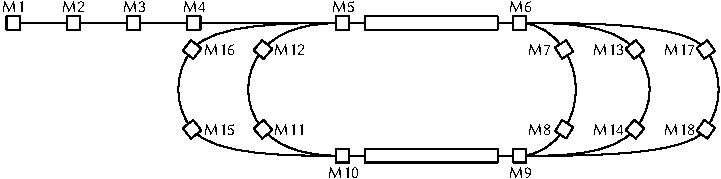
\includegraphics{Layouts/layouts-02}
  \caption{A recirculator illustrates particles traveling
           through a varying sequence of magnets.}
  \label{fig:accel.CEBAF}
\end{figure}

A linked list of \emph{magnets} cannot properly represent the
physics of this situation. In a linked list, magnet \ptcelm{M6},
for example, must point to only one magnet. It cannot point to
\ptcelm{M7}, \ptcelm{M13}, \emph{and} \ptcelm{M17} unless we
create two clones of \ptcelm{M6}. Creating clones, however, is
a bad idea: If we wish to adjust the position or strength of
magnet \ptcelm{M6}, such adjustments would have be made three
times: once in the magnet itself, and once in each of its two
clones.

\index{linked list!example for fibres}
\index{fibre!defined}
%
A better solution separates the magnets from the linked list that
tracks the path of particles through the magnets. \PTC\ does this
with a linked list of containers called \emph{fibres}, each with
a pointer to the appropriate magnet. Adjustments to the position
or strength of a magnet are made once and are automatically taken
into account each time a container in the linked list points to
that magnet. We discuss the linked list of containers with pointers
to magnets in \TSref*{accel.topo}.

\begin{figure}[ht]
  \centering
  %\includegraphics[width=.65\textwidth]{illustrations/model-RHIC}
  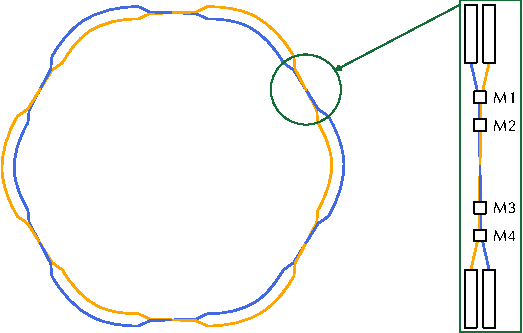
\includegraphics{Layouts/layouts-06}
  \caption{Particles circulating in different directions
           through an accelerator.}
  \label{fig:accel.RHIC}
\end{figure}

\index{accelerator topology!collider}
\index{collider!example}
\index{Relativistic Heavy Ion Collider!example based on}
\index{RHIC|see{Relativistic Heavy Ion Collider}}
\index{Brookhaven National Laboratory!example based on}
\index{forward propagation!example}
\index{backward propagation!example}
%
What about a collider? \fref[c]{accel.RHIC}, based on the intersecting
rings of the Relativistic Heavy Ion Collider (\RHIC) at Brookhaven
National Laboratory (\BNL), shows particles circulating in both
directions (forward and backward propagation) through some of the
same magnets. For example, the particles following the blue path go
though one set of magnets in the sequence \ptcelm{M1}, \ptcelm{M2},
\ptcelm{M3}, \ptcelm{M4}. Meanwhile, the particles following the
yellow path traverse the same set of magnets in the reverse order:
\ptcelm{M4}, \ptcelm{M3}, \ptcelm{M2}, \ptcelm{M1}.

\index{linked list!example for fibres}
%
Using an array or a linked list with clones of magnets creates
the same problems as before, and \PTC\ alleviates the difficulties
by using doubly-linked lists%
\marginnote{The use of a \emph{doubly}-linked list enables both
forward and reverse propagation through a given sequence of
beamline elements.}
of containers that follow the particle
paths---containers which have inside them pointers to the appropriate
magnets. Changes to the strength or position of, say, magnet
\ptcelm{M3} are made once in the object for magnet \ptcelm{M3} and
are immediately reflected in the two linked lists---one linked list
for each of the two particle beams.


\section{Modeling Accelerator Topologies}
\label{sec:accel.topo}

\index{accelerator!modeling}
\index{modeling!accelerator topologies}
%
\glossary{accelerator topology}{A description in spatial terms of
the magnets in an accelerator and how they interact with particles.}
%
To set up a linked list of containers with pointers to the elements
in a beamline, \PTC\ employs three different data types:
\ptctyp{element}, \ptctyp{fibre}, and \ptctyp{layout}.
\PTC\ also provides what it refers to as a \emph{\DNA\ database},
which one may populate with \ptctyp{layout}s that one may use to
construct complex accelerator topologies. Finally, for the proper
positioning of elements in the accelerator, \PTC\ uses two additional
data types: \ptctyp{chart} and \ptctyp{patch}. We discuss all these
concepts in this section.


\subsection{Element}

\index{element!defined}
\index{data type!\ptc{ELEMENT}}
\index{ELEMENT@\ptc{ELEMENT}!data type}
\index{type|see{data type}}
%
The data type \ptctyp{element} represents a beamline element in a
machine. It contains information about the element type (dipole,
quadrupole, rf cavity, \etc), its physical properties (length,
strength, \etc), and its location and orientation in space.  In
\PTC, it is the fundamental object. \PTC\ preserves each element's
physical and mathematical integrity to ensure that it can be
positioned, repositioned, or misaligned \emph{as a whole}. At the
same time, \PTC\ provides the capability for one to look inside the
element to see, for example, details of a particle trajectory. One
should therefore \emph{never} feel compelled to split an element in
half. \et{In \PTC\ one can simply choose an even number of integrations steps; the code automatically sets up a pointer called tm that points to the center of the magnet. }

In addition to information about the element itself, the data type
\ptctyp{element} includes information about which \ptctyp{fibre}s
point to it. This information is used by \PTC\ to ensure that if
an element is moved, then all beamlines containing it know about
the move.

%As in a real machine, the same element may appear in several
%beamlines, or it may reappear in the same recirculating beamline
%several times.


\subsection{Fibre}
\fxnote{Add margin note re origin of term \emph{fibre}.}

\index{fibre!defined}
\index{data type!\ptc{FIBRE}}
%
The data type \ptctyp{fibre} contains a pointer to a beamline
element as well as pointers to the fibres that precede and follow
it along a particle path. When strung together in a linked list,
a sequence of fibres defines a beamline. The fact that different
fibres can point to the same element means that separate beamlines
can share common elements; and this gives \PTC\ the capability to
model complex accelerator topologies.

\index{chart!defined}
\index{patch!defined}
%
A \ptctyp{fibre} contains, among other items,
\begin{itemize}
  \item a pointer to an \ptctyp{element};
  \item pointers to the previous and next \ptctyp{fibre}s
        along a beamline;
  \item a pointer to a \ptctyp{chart} that locates the element
        within the global reference frame;
  \item a pointer to a \ptctyp{patch} that connects the elements
        of successive fibres geometrically, energetically, and
        temporally;
  \item the \emph{direction of propagation} through the element.
\end{itemize}


\subsection{Layout}

\index{layout!defined}
\index{beamline!defined as layout}
\index{data type!\ptc{LAYOUT}}
%
The data type \ptctyp{layout} represents a beamline as a doubly-linked
list of \ptctyp{fibre}s. It follows the particle path by specifying
the order of the fibres, which each point to an actual element in
the beamline.%
\sidenote{Note that a \ptctyp{layout} need not represent an entire
machine: it may represent just a piece of an machine. The full
accelerator would then be built from several layouts.}
In addition, a \ptctyp{layout} defines the direction of
propagation through the sequence of fibres and whether the particles
recirculate.

\begin{figure}[ht]%\forcerectofloat
  \centering
  %\includegraphics[width=.9\textwidth]{illustrations/model-JLAB-fibres}
  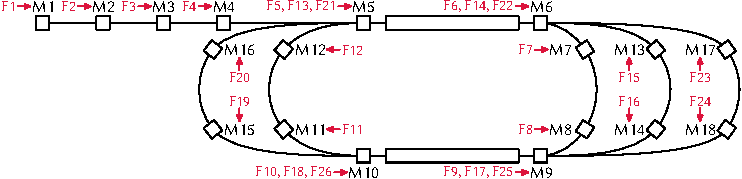
\includegraphics{Layouts/layouts-03}
  \caption{A layout with a linked list of fibres pointing to magnets.}
  \label{fig:CEBAF.layout.fibres}
\end{figure}

As an example,%
\marginnote{As before, we say ``magnet'', but it may mean any type
of beamline element.}
consider the accelerator illustrated in
\fref{accel.CEBAF}. We could construct it as indicated in
\fref{CEBAF.layout.fibres}, which shows a \PTC\ \ptctyp{layout}
with a linked list of 26 fibres (\ptcelm{F\#}) pointing to the
18 magnets (\ptcelm{M\#}).

\index{DNA database!defined}
\index{database|see{DNA database}}
\index{DNA sequence!defined}
\index{sequence|see{DNA sequence}}
\index{DNA|see{DNA array, DNA database, \emph{or} DNA sequence}}
%
\newthought{Most accelerator modeling codes} do not, as \PTC\ does,
enforce a dichotomy between fibres and elements. As a consequence,
it can be difficult to import lattice descriptions from other codes
into \PTC\ in a manner consistent with \PTC's approach to modeling
accelerators. To overcome this difficulty, \PTC\ provides what it
refers to as a \emph{\DNA\ database}. This database is first
populated with a set of \ptctyp{layout}s whose fibres point to
unique elements.  In other words, no element appears more than
once---via the fibres---in the set of \DNA\ layouts. (This much may,
if desired, be done by importing from an external lattice description.)
These simple layouts---we shall refer to them as
\emph{\DNA\ sequences}---may then be used to construct complex layouts
of the form shown in \fref{CEBAF.layout.fibres}.

\begin{marginfigure}[-2\baselineskip]
  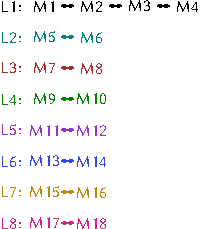
\includegraphics{Layouts/layouts-04}\vspace{5pt}
  \caption{DNA database with eight DNA sequences (\ptcelm{L1}
           through \ptcelm{L8}). The arrows represent the links in
           the doubly-linked list of fibres that constitutes a layout.
           Each fibre points to (contains) the indicated magnet
           (\ptcelm{M1}--\ptcelm{M18}).}
  \label{fig:DNA.database}
\end{marginfigure}
%
\index{layout!non-trackable}
%
As a concrete example, consider how we might do this for the
accelerator shown in \fref{accel.CEBAF} or \fref*{CEBAF.layout.fibres}:
We first create a set of layouts in which no magnet appears
twice, and which have no magnets in common. The logical course
in this case is to create the eight layouts \ptcelm{L1} through
\ptcelm{L8} shown in \fref{DNA.database}. Note that each of the
eighteen magnets appears just once in this database. Here we show
each of the \DNA\ sequences in a different color; and these colors
match those used in \fref{CEBAF.DNA}, which shows the accelerator
with the different \DNA\ sequences indicated by the corresponding
colors.

\begin{figure}[ht]%\forceversofloat
  \centering
  %\includegraphics[width=.9\textwidth]{illustrations/model-JLAB-DNA}
  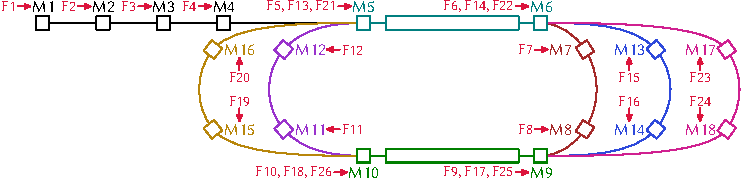
\includegraphics{Layouts/layouts-05}
  \caption{Eight layouts or DNA sequences.}
  \label{fig:CEBAF.DNA}
\end{figure}

\index{layout!trackable}
%
Having created the eight \DNA\ sequences in our \DNA\ database,
we can now use \PTC\ to string these basic layouts together to
create the \emph{trackable layout} that represents the full machine
illustrated in \fref{accel.CEBAF}, or \fref*{CEBAF.layout.fibres}
or \fref*{CEBAF.DNA}. Evidently, a trackable layout may be constructed
from one or more \DNA\ sequences.%
\sidenote{By contrast, we may sometimes refer to the
\DNA\ sequences---high-level building blocks of our accelerator
model---as \emph{non-trackable layouts}.}

In general, once we have populated the \DNA\ database (either
from within \PTC\ or by importing external lattice descriptions) we
can use \PTC\ to string together these basic layouts to create
the additional layouts we need for tracking. These latter---\ptcelm{T1}
through \ptcelm{TN}, say---contain fibres that point to elements
in the \DNA\ database. For the recirculator shown in
\fref{accel.CEBAF}, we would create one beamline layout \ptcelm{T1}
with 26 fibres, each pointing to an element in the \DNA\ database.
For the collider shown in \fref{accel.RHIC}, we would create two
beamline layouts, \ptcelm{T1} and \ptcelm{T2}, one layout for
each ring.


\subsection{Chart and Patch}
\label{sec:chart.patch}

\index{patching!reference frames}
\index{reference frame!patching}
\index{geometric transformation!patching}
\index{tracking!automatic}
%
\PTC\ uses  the new data types \ptctyp{chart} and \ptctyp{patch}
to locate, connect, and move the elements of a beamline. The
generic capability, which we term \emph{patching}, connects the
exit frame of one element to the entrance frame of the subsequent
element.

\index{chart!defined}
\index{chart!contains misalignment}
\index{data type!\ptc{CHART}}
%
The data type \ptctyp{chart} contains a pointer to a frame of
reference (actually the collection of three frames illustrated in
\fref{LEGO.element}) that locates a fibre (really the element the
fibre points to) within \PTC's global three-dimensional reference
frame. The chart also contains information that describes, if present,
any misalignment of the fibre.

\index{patch!defined}
\index{data type!\ptc{PATCH}}
%
The data type \ptctyp{patch} contains information about the
about the relation between the exit reference frame of one
element and the entrance reference frame of the subsequent
element. As a consequence, a \ptctyp{patch} is a property not
of an \ptctyp{element} but of a \ptctyp{fibre}, and it must
be computed \emph{after} placing both elements in their final
locations.

As a concrete example, consider the set of elements illustrated
in \fref{patch.elems}. There we see three elements separated by
a pair of drifts. We know the locations of these elements
(in particular the reference frames attached to these elements)
because of the information stored in the corresponding charts.
The second drift is explicitly defined as the third beamline
element. The first drift, however, is not explicitly defined.
The exit frame of element~1 and the entrance frame of element~2
do not coincide, and this indicates the need for a patch. The
remaining elements all have exit-entrance frame pairs that
coincide, and hence no additional patches are required.

\begin{figure}[ht]%\forcerectofloat
  \centering
  %\includegraphics[width=.9\textwidth]{illustrations/patching-element}
  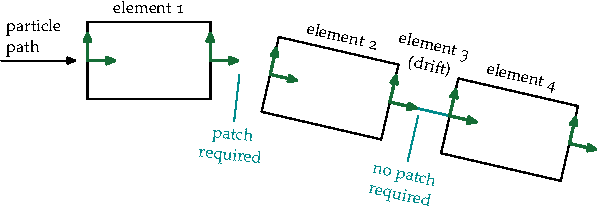
\includegraphics{Patches/patches-01}
  \caption{Patching elements in a single beamline.}
  \label{fig:patch.elems}
\end{figure}

\index{recirculator!patching beamlines}
%
As another example of patching, \fref{patch.recirc} shows three
magnets in a recirculator. A high-energy particle passing through
magnet~1 follows the red trajectory to magnet~2. After exiting
magnet~2, the particle continues around the machine and returns
with a lower energy (after deceleration by appropriately phased
rf fields) to magnet~1. Because the particle has less energy,
magnet~1, the separator, now bends it along the blue trajectory
towards magnet~3, the first magnet in a new beamline.
Magnet~1 of \fref{patch.recirc} must, of course, appear in two
fibres: the first points to magnet~2 as the subsequent element,
while the second points to magnet~3. What about the patches?
Assuming the exit frame of magnet~1 and the entrance frame of
magnet~2 have the same unit vectors but different origins. then
the patch between the fibres pointing to magnets 1 and 2 must
correspond to a simple drift of the appropriate length---and that
is exactly what \PTC\ will compute. The patch between the fibres
pointing to magnets 1 and 3 corresponds to three actions: a drift
of length $d$, a co\"ordinate frame rotation by angle $\alpha$,
and a translation of length $h$.

\begin{figure}[ht]
  \centering
  %\includegraphics[width=.7\textwidth]{illustrations/patching-beam-lines}
  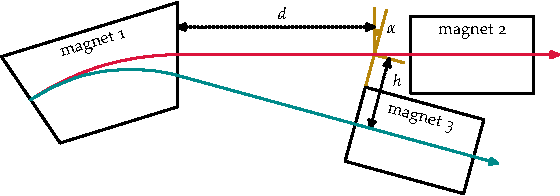
\includegraphics{Patches/patches-02}
  \caption{Patching elements in multiple beamlines.}
  \label{fig:patch.recirc}
\end{figure}


\subsection{Misalignments}

\index{misalignment!described}
%
The accelerator we design is never the one we build. This fact
makes it essential to investigate the margin for error in any
design. To simulate misalignment errors, \PTC\ uses the approach
illustrated in \fref{misalignment}. There we show the original
element~2 with a light gray outline, and the misaligned element~2
with a red outline. To push a particle from the exit of element~1
to the entrance of element~3, \PTC\ first applies the patch from
element~1 to the original element~2. Then \PTC\ traverses element~2
in three steps: an entrance misalignment, the standard element~2,
and an exit misalignment.
\PTC\ then applies the patch from element~2 to element~3.
If we remove the misalignment (which translates and rotates element~2),
the element returns to its design position in the fibre.

\begin{figure}[ht]%\forceversofloat
  \centering
  %\includegraphics[width=.9\textwidth]{illustrations/misaligning-element}
  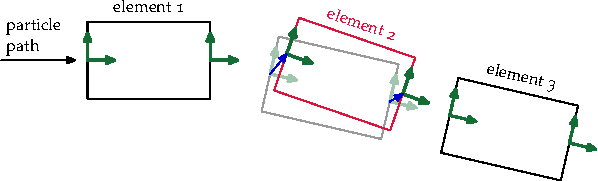
\includegraphics{Patches/patches-03}
  \caption{Misaligning an element.}
  \label{fig:misalignment}
\end{figure}


\section{Analyzing an Accelerator to Understand its Properties}
\label{sec:analyze.accel.prop}

\index{accelerator!analysis}
\index{accelerator!properties}
\index{property!accelerator}
%
In this overview chapter, the first two sections,
\Tref{sec:track.ptcl.accel} and \Tref{sec:accel.topo}, discuss
the essential concepts and data structures used by \PTC\ to
construct a computer model of an accelerator and simulate particle
trajectories through that model. Your next activity is likely to
be that of asking questions of your simulated accelerator: Where
is the particle in that magnet? What are the Twiss parameters at
this location in the ring? What are the horizontal and vertical
tunes of this machine? How much synchrotron radiation does my
particle emit while traversing this magnet? Such questions are
the domain of \emph{analysis}.

\index{map-based methods!global}
%
At the heart of the software design decisions made for \PTC\ lies
the desire to analyze \emph{real} accelerators. The fact that real
accelerators are complicated beasts---with many individual magnets
performing many individual functions---leads directly to \PTC's
simulating accelerators using the \LEGO-block approach, which
emphasizes a \emph{local} view of beamline elements and particle
tracking. Similarly, the desire to analyze leads directly to \PTC's
use of map-based methods, which emphasize a \emph{global} view of
the accelerator.

\index{map-based methods}
\index{one-turn map}
\index{perturbation theory!derived via one-turn map}
%
Map-based methods are fundamental to the analysis of real
accelerators. Think of a one-turn map as a piece of sophisticated
diagnostic hardware that you install at some point in the ring.
It enables you to observe the beam turn after turn. It follows that
any \emph{sensible} question you might ask about the beam at that
point in the ring must be contained within that one-turn map.
Indeed, all of standard perturbation theory may be expressed
entirely in terms of the one-turn map.\cite{Forest:1990:HamFree}

If you desire information at some other point in the ring, then
you must, of course, install another sophisticated beam monitor
at that new location. Using map-based methods, this will be
equivalent to a proper combination of the one-turn map at your
original location and the transfer map that connects the two
locations of interest. As a consequence, a one-turn map plus
partial-turn transfer maps contain the answers to all sensible
questions you might ask of an accelerator model.

\index{one-turn map!analysis independent of construction}
%
The analogy of a one-turn map as a sophisticated beam monitor
also implies---quite correctly---that no connection exists
between the \emph{construction} of a one-turn map and its
\emph{analysis}. The construction is done using a strictly
local approach, which is our only hope of getting the physics
right in this complicated and messy world. Once we've obtained
the one-turn map, we may forget where it came from and what
various frames of reference were used to compute it. We now
concentrate on asking sensible questions of our ``beam monitor''.


\subsection{Local versus Global Information}

\index{local information!analysis}
\index{global information!analysis}
\index{property!local}
\index{property!global}
\index{local information|see{\emph{also} local property}}
\index{global information|see{\emph{also} global property}}
%
\PTC\ provides you with two kinds of information: local and global.

\index{local information!defined}
%
Information about an element, or a particle in an element,
is called \emph{local} if it can be obtained independently of
any knowledge of the element's position in an accelerator.
It could be obtained even if the element were a prototype
sitting on a test bench in your lab. The field strength at
a particular location in the element is an obvious example
of local information. Another example is a particle's
trajectory through a magnet: When, for example, an electron
appears at the entrance of a quadrupole, we can predict its
(local) trajectory without any knowledge of where the electron
came from, or where it is going. Yet another example of local
information is the amount of synchrotron radiation emitted by
a particle as it traverses a magnet.

\index{global information!defined}
%
Information is called \emph{global} if it can be obtained
only after constructing an accelerator. The dynamic aperture
is an example of global information, because it makes sense
only in the context of circulating particles around an
accelerator ring. Other examples include\\
%\vspace{-\baselineskip}
\begin{tabular}{lll}
  tune          & closed orbit            & normal mode decomposition \\
  tune shift    & resonance               & damping partition number \\
  chromaticity  & linear lattice function & nonlinear distortion
                                               function \\
  anharmonicity & equilibrium emittance   & short-, mid-, and
                                               long-term stability
\end{tabular}\\
%\vspace{-\baselineskip}
\noindent and much more.

Note that all local quantities are governed solely by the
particulars of an element and the underlying equations of
motion. Particle information, local field strengths, and the
Lorentz equation are all you need to know for the computation
of local quantities. Global quantities, on the other hand,
are governed by the fact that an accelerator ring is designed
to circulate particles in stable orbits for many turns. They
result from our efforts to \emph{interpret} the one-turn map.


\subsection{Polymorphs and Normal Form}

The simplest simulation of particle trajectories in an accelerator
represents a particle as an array $z$ of real numbers, which
constitutes the phase-space co\"ordinates and any other quantities
(spin, for example) that need to be tracked. One then tracks the
particle through the accelerator by integrating the appropriate
equations of motion with initial conditions given by $z^i$. If we
wish to know the behavior of nearby particles, then we could, of
course, launch other particles with initial conditions $z^i+\varepsilon$
and study how the results vary with $\varepsilon$. What we want,
then, is a functional representation of the behavior near $z^i$
using, for example, a Taylor series. Moreover, it will be convenient,
indeed desirable, if we can switch between the real or Taylor series
representations at runtime. To achieve this, \PTC\ defines the
variable type \ptctyp{real\_8}, which holds containers for a real,
a Taylor series, and other information, as well as a flag that
allows the user to set the representation. This \ptctyp{real\_8}
is a so-called \emph{polymorphic} variable. With this polymorphism,
\PTC\ gives us access to all of standard perturbation theory,
including the kinds of global information mentioned above.
To make the most effective use of polymorphism, \PTC\ also overloads
the standard mathematical operators so that algorithms written for
reals immediately apply to Taylor series and any other representations
held by the type \ptctyp{real\_8}.

As indicated above, rather than propagating a particle,
\ie\ a \ptctyp{real}, through an accelerator, one may instead wish
to propagate a \emph{neighborhood}, \ie\ an array of truncated power
series (\TPS) that represents the particle and its phase-space
neighborhood. Given a software library that implements a truncated power
series algebra (\TPSA), one can use polymorphism and operator
overloading to turn any single-particle tracking algorithm into a
map generation algorithm.
The polymorphism of \PTC\ makes it possible to to compute transfer
maps in a transparent manner.
%The result
%of such tracking is a one turn map for that region of phase space.

\index{SDGQ@\SDGQ\ ($s$-dependent global quantity)}
\index{$s$-dependent global quantity!defined}
%
\newthought{The concept of a {normal form}} is absolutely central
to the modern view of accelerator analysis. In the very simplest
case, a one-turn map reduces to a matrix $M$, and we factor it in
the form of a similarity transformation:
\begin{equation*}
  M = A \cdot N \cdot A^{-1}.
\end{equation*}
Here $N$ denotes a \emph{normal form}, and $A$ denotes the matrix
that transforms between $N$ and $M$. Continuing our simplest example,
$N$ generates rotations in each of the separate phase planes,
and $A$ converts the circles of normal form co\"ordinates to
generic phase-space ellipses. If we go to another location in the
accelerator, the one-turn map will differ, but it will have the
same normal form:
\begin{equation*}
  M' = A' \cdot N \cdot A'^{-1}.
\end{equation*}
In other words, $N$ is an invariant of the ring.
Global scalars, by which we mean global quantities that do not
depend on location around the accelerator, may be derived from
$N$. The $s$-dependent global quantities (\SDGQ{}s) may be derived
from the transformations $A$, $A'$, \dots.
Thus, for example, one extracts tunes from $N$ and linear lattice
functions from the $A$s.

Two very important benefits derive from a normal form factorization
of the one-turn map: The first benefit is that this factorization
generalizes in a straightforward manner to nonlinear maps. We may
thus write the map $M(z)$ as the composition
\begin{equation}\label{eq:M.ANAi}
  M(z) = A \circ N \circ A^{-1}(z),
\end{equation}
where now $M$, $A$, and $N$ all denote nonlinear functions on phase
space. As in the matrix case, the normal form $N(z)$ yields the
global scalars, and the transformation $A(z)$ yields the \SDGQ{}s.
$N$, for example, contains not only the tunes, but also the nonlinear
information of how the tunes vary with amplitude. The second benefit
is that we may use the \emph{same code} that produced the one-turn
map $M(z)$ to propagate the normalizing transformation $A(z)$. Doing
exactly this---using the polymorphic capabilities of \PTC, of
course---we can compute \SDGQ{}s at many locations around the ring.

As with all things wonderful, some caveats attach to the normal
form decomposition \eqref{M.ANAi}. The first caveat is associated
with the approximate nature of the work we do. Unless our system
is extremely special, we can know $M(z)$ only up through some
finite order. Moreover, because of the complicated nature of
particle orbits in accelerators, the expansion is generally
asymptotic. As a consequence, we should examine all analyses in
the light of common sense and actual particle tracking.%
\sidenote{This should \emph{already} be part of your routine.}

The second caveat is associated with the fact that the
transformation $A(z)$ is not unique: If $B$ denotes any
transformation that commutes with $N$, then replacing $A(z)$ in
\eqref{M.ANAi} with $A \circ B(z)$ yields the same result. In
other words, the particular $A$ we choose to work with depends on
certain conventions. For physical quantities associated with $A(z)$,
this freedom in the definition of $A$ necessarily has no effect. But
some quantities%
\sidenote[][-2\baselineskip]{One example is the so-called phase
advance. Consider two locations in the ring that have identical
one-turn maps. At such so-called \emph{matched} locations in a ring, the normalizing
transformations (chosen with common conventions!) are identical;
as a consequence, the phase advance between such locations is
well-defined. Between \emph{un}matched locations, however, the
definition of phase advance can depend on the conventions used in
extracting the $A$s.}
that people discuss \emph{do}, in fact, depend on the particular
choice for the normalizing transformation $A$. Such quantities,
needless to say, cannot be physical and should be used with great
care, or not at all.\cite{Chao:2008:SLIMrevisted}


\section{Modeling Particle Interactions}
\label{sec:ptcl.intxns}

\index{particle!interaction}
\index{modeling!particle interactions}
%
This overview chapter has, until now, discussed concepts related
to single-particle dynamics. In this section we introduce some
concepts related to the inclusion of particle interactions in
\PTC\ simulations. Some of these concepts, however, apply also
to single-particle dynamics, and hence we urge even readers not
interested in space-charge to at least skim this section.

We begin with a caveat: \emph{The inclusion of particle
interactions violates the philosophy of \PTC.} To see
this, consider a beam of self-interacting particles at
a moment when the head has entered a magnet and the tail
has not. Particles in the head and tail communicate via
the self interactions, and hence the dynamics of particles
in the head and tail affect one another. If we place the
magnet in a different location, particles in the head will
follow different trajectories. The particle interactions
communicate this information to the tail, and now particles
in the tail also follow different trajectories---their
behavior differs because of a change in a magnet they have
yet to see. This scenario tells us that if our beam is
spatially extended and self-interacting, we cannot define
an isolated propagator for each element. In other words,
particle interactions violate the \LEGO-block approach to
modeling accelerators.

To fit within the philosophy of \PTC, beamline elements must
be independent of one another. This idealization---upon which
most tracking codes rely---should be borne in mind when using
\PTC---or any of those other codes---to simulate beams with
self-interacting particles.%
\sidenote{Overlapping fringe fields also violate the principle
of magnet independence; and in that case, too, one must exercise care.}

\makeusother
In the rest of this section, we discuss some of the data
types useful for including particle interactions:
\ptctyp{integration_node}, \ptctyp{node_layout}, \ptctyp{probe},
and \ptctyp{temporal_probe}. We also describe the basic idea
behind the time-based tracking capability of \PTC.


\subsection{Integration Node}
\label{sec:integr.node}

\index{integration node!defined}
\index{data type!\ptctyp{integration\_node}}
\index{element!composed of integration nodes}
\index{node|see{integration node}}
\index{entrance patch!integration node}
\index{entrance fringe field!integration node}
\index{exit patch!integration node}
\index{exit fringe field!integration node}
\index{fringe field!integration node}
%
The data type \ptctyp{integration\_node} represents a step of
integration in \PTC. In particular, this data type includes
entrance and exit reference frames, pointers to the previous
and next integration nodes along a particle path
(see \Tref{sec:node.layout}), and a pointer to the parent
\ptctyp{fibre} that contains it. Integration nodes allow us to
examine data inside a beamline element without violating the
element as a fundamental unit---a self-contained \LEGO\ block.
They allow us to resist the temptation to ``slice'' an element
by hand: they \emph{are} the slices. The data type
\ptctyp{integration\_node} also contains an integer that
determines the \emph{type} of integration node, of which there
are five. See \fref{integr.nodes}. On traversing the integration
nodes that represent an element, one encounters, in order,
\begin{itemize}
  \item an entrance patch (and misalignment, if any), which
connects the geometry described by the fibre to that of the
preceding fibre in the linked list;
  \item an entrance fringe field, which contains approximate
fringe effects (if any);
  \item $N$ body integration nodes representing the body of element;%
\footnote{The choice of $N$, which you are free to modify,
obviously affects the accuracy of your simulation.
\Cref[c]{symplectic.integ} discusses how to split elements into
integration nodes.}
  \item an exit fringe field, which contains approximate fringe
effects (if any);
  \item an exit patch, which connects the geometry described by
the fibre to that of the following fibre in the linked list.
\end{itemize}



\begin{figure}[ht]
  \centering
  %\includegraphics[width=.9\textwidth]{illustrations/integration-nodes}
  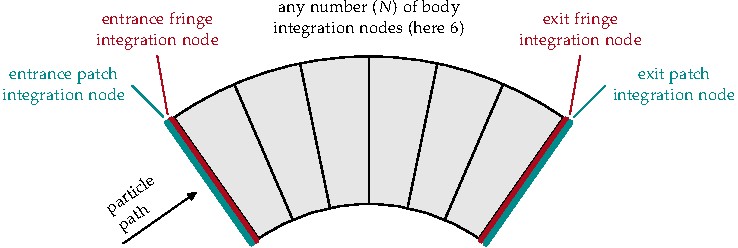
\includegraphics{Elements/nodes-01}
  \caption{$N+4$ integration nodes cover an element.}
  \label{fig:integr.nodes}
\end{figure}

\index{s-based tracking!integration node}
\index{time-based tracking!integration node}
%
Using $s$-based tracking, we can obtain particle data at the
entrance and exit of each integration node in the body of a
magnet, that is, at the seven black lines in \fref{integr.nodes}.
In addition, we can obtain first-order information about the location
within a node of a particle at some fixed time
(see \Tref{sec:pseudo.time}).

The integration nodes \emph{contain no duplicate data about
the elements}; they have no existence apart from the beamline
elements they represent. Because the data in the integration
nodes reside on the fibres (which point to the elements),
\PTC\ is able to carry over changes affecting elements
(\eg, a change in the magnetic field) and changes affecting
the fibres (\eg, misalignments) to the integration nodes.


\subsection{Node Layout}
\label{sec:node.layout}

\index{node layout!defined}
\index{data type!\ptc{NODE\_LAYOUT}}
\index{layout|see{\emph{also} node layout}}
\index{linked list!integration nodes}
\index{beamline!expanded}
%
\fxnote{Should have some comment, probably later about
\ptctyp{node\_layout} inserting a bunch of additional reference
frames.}
%
The data type \ptctyp{node_layout} represents a beamline as a
linked list of \ptctyp{integration_node}s. It includes pointers
to the first and last integration nodes in the beamline, as well
as a pointer to the parent \ptctyp{layout}. To access the
integration nodes of a particular fibre, one may step through
them, making use the fact that the data type \ptctyp{fibre}
includes pointers to the first, last, and middle integration nodes
for the corresponding element.

A \ptctyp{node_layout} is not created automatically when you
create a \ptctyp{layout}: You must ask \PTC\ to create it and
populate the associated reference frames.
\fxnote{Add reference to example(s).}


\subsection{Probe and Temporal Probe}

\index{probe!defined}
\index{data type!\ptctyp{probe}}
%
The data type \ptctyp{probe} represents a particle. In particular,
it contains, for a given particle, both the orbital phase-space data
and a \ptctyp{spinor} for the spin data. Should the particle become
lost, the \ptctyp{probe} contains a \ptctyp{logical} in which to
record this fact, as well a pointer to the \ptctyp{integration_node}
in which the particle loss occured.

\index{temporal probe!defined}
\index{data type!\ptc{TEMPORAL\_PROBE}}
\index{probe|see{\emph{also} temporal probe}}
%
The data type \ptctyp{temporal_probe} contains a \ptctyp{probe}
together with information relevant to the time-based tracking
capability of \PTC. This includes a pointer to the
\ptctyp{integration_node} that currently contains the particle.
\makeussubscript


\subsection{Time-based Tracking}
\label{sec:pseudo.time}

\index{time-based tracking!integration node}
\index{time-based tracking!described}
%
Any high-order $s$-based integrator may be converted to a
first-order time-based integrator \emph{provided information
is available about the three-dimensional environment.} When
we ask \PTC\ to perform time-based tracking, \PTC\ augments
its $s$-based information with temporal information. \PTC's
tracking remains fundamentally $s$-based, but with the
additional information, it can determine which integration
node a particle is in at a given time. \PTC\ can
then compute a first-order accurate location inside that node
for the particle at that time.

\begin{figure}[ht]
  \centering
  %\includegraphics{illustrations/space-charge-kick}
  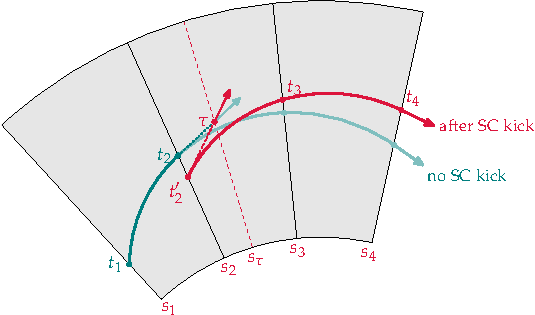
\includegraphics{Elements/nodes-02}
  \caption{Applying a space-charge kick at time $\tau$.}
  \label{fig:sc.kick}
\end{figure}

\index{space-charge kick!used with time-based tracking}
\index{kick!space-charge}
\index{particle!space-charge kick}
\index{particle!interaction}
\index{space-charge kick!applying}
%
\PTC's time-based tracking capability allows us to obtain a
snapshot of the beam at a fixed time. \fref[c]{sc.kick}
illustrates this approach to applying a space-charge kick at
time $\tau$:
\begin{enumerate}
  \item \PTC\ checks node by node the entrance and exit times
of a particle to determine the integration node for which
$\tau \in [t_\text{entrance},t_\text{exit})$. After locating
the appropriate node, \PTC\ returns the particle to the node
entrance. At this point in \fref{sc.kick}, because $\tau$ falls
between times $t_2$ and $t_3$, the particle is on the blue curve
at the point labeled with time $t_2$.
  \item \PTC\ determines the time difference
$\delta t = \tau - t_\text{entrance}$. Then, using the particle's
position and momentum at the node entrance as an initial condition,
and assuming the current integration node to be a drift,
\PTC\ computes a position and momentum for the particle at time $\tau$.
It records the shift $\delta s$ in the \ptctyp{temporal\_probe}.
If the element \emph{is} a drift, the position of the particle at
time $\tau$ is exact. If the element is \emph{not} a drift, the
position of the particle at time $\tau$ is a close approximation.
At this point in \fref{sc.kick}, the particle is at the point
labeled with time $\tau$.
  \item After completing the above two steps for all particles in
the beam, you can apply space-charge kicks to your particles. At
this point in \fref{sc.kick}, the particle remains at the point
labeled with time $\tau$, but it has a new momentum, as indicated
by the angle between the light blue arrow and the red arrow.
  \item \PTC\ now drifts the particle---with its new momentum---back
to the entrance of the integration node. At this point in
\fref{sc.kick}, the particle is back in the $s_2$ plane, but now
on the red curve at the point labeled with time $t_2'$.
  \item \PTC\ now continues tracking the particle---with its new momentum---seeking the integration node for which $t_\text{entrance}$ and $t_\text{exit}$ bracket the time for the next space-charge kick.
\end{enumerate}

\endinput
